\documentclass[mathserif]{beamer}
\usepackage[ngerman]{babel}
\usepackage[latin1]{inputenc}
\usepackage{amsmath, amssymb}
\usepackage{latexsym}
\usepackage{tikz}
\usepackage{multicol}
\usetikzlibrary{calc}

%
\newcommand{\R}{\mathbb{R}}
\usetheme{Madrid}
\usecolortheme{seahorse}
%
%
\usepackage{graphicx}
\graphicspath{{.}{./neurons}}


\title[MNS Project 2]{MNS Project 2: Learning of Grid Cells}
\author[C.Lang, C.E.Sezener, C.Winklmayr]{Claus Lang, C. Eren Sezener and Claudia Winklmayr}
\institute{BCCN}
\date[9.2.2016]{February $9^{th}$ 2016}
%
\begin{document}
\maketitle
%
%
%
\begin{frame}
\frametitle{Structure}
	\begin{itemize}
	\item Introduction\newline
	\item Modelling details\newline
	\item Results
	\end{itemize}
\end{frame}
%
%
%
\begin{frame}
\frametitle{Introduction}
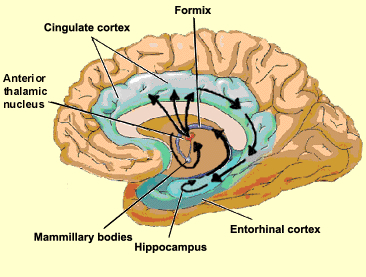
\includegraphics[width=0.7\textwidth]{mEC.jpg}\newline
%http://www.irafs.org/images/irafs_nl_eng_2_files/image007.jpg
In Hippocampus and the medial enthorhinal cortex (mEC) several types of neurons have been found to encode an animals spacial location.  
\end{frame}
% 
%
%
%\begin{frame}
%\frametitle{Cells encoding spacial location}
%\begin{itemize}
%\item \textbf{Place cells} \newline
%%Located in hippocampus. Activated when the animal enters a specific region of the environment - the \textit{place field]}. \newline
%%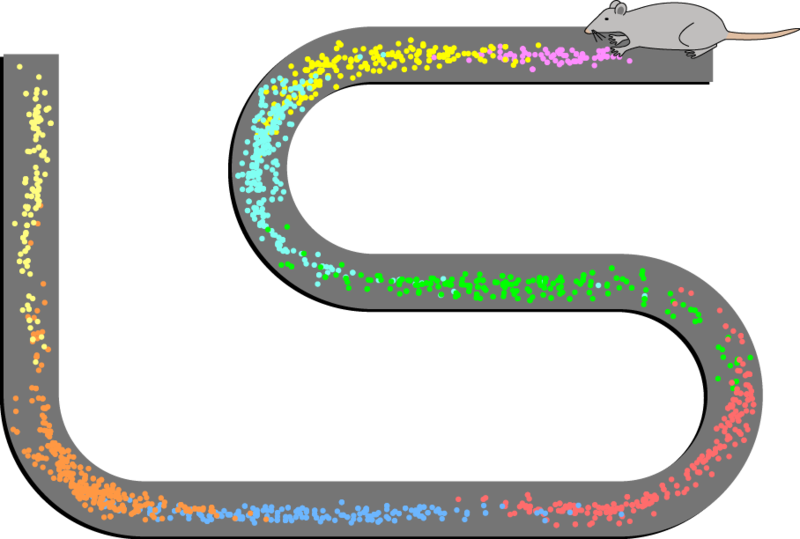
\includegraphics[width=0.33\textwidth]{Place_Cell_Spiking_Activity_Example.png}
%%"Place Cell Spiking Activity Example" by Stuartlayton at English Wikipedia. Licensed under CC BY-SA 3.0 via Commons - https://commons.wikimedia.org/wiki/File:Place_Cell_Spiking_Activity_Example.png#/media/File:Place_Cell_Spiking_Activity_Example.png
%\item \textbf{Grid cells} \newline
%%Located in  medial enthorhinal cortex (mEC). Activated at several spacial positions. The firing map shows an equally spaced hexagonal pattern. \newline
%\item \textbf{Head-direction cells}\newline
%\item \textbf{Head-Grid-Conjunctive cells}
%\end{itemize}
%\end{frame}
%
%
%
\begin{frame}
\frametitle{Place cells}
  \begin{columns}[T]
    \begin{column}{.5\textwidth}
			Located in hippocampus. Activated when the animal enters a specific region of the environment - the \textit{place field}.
    \end{column}
    \begin{column}{.5\textwidth}
    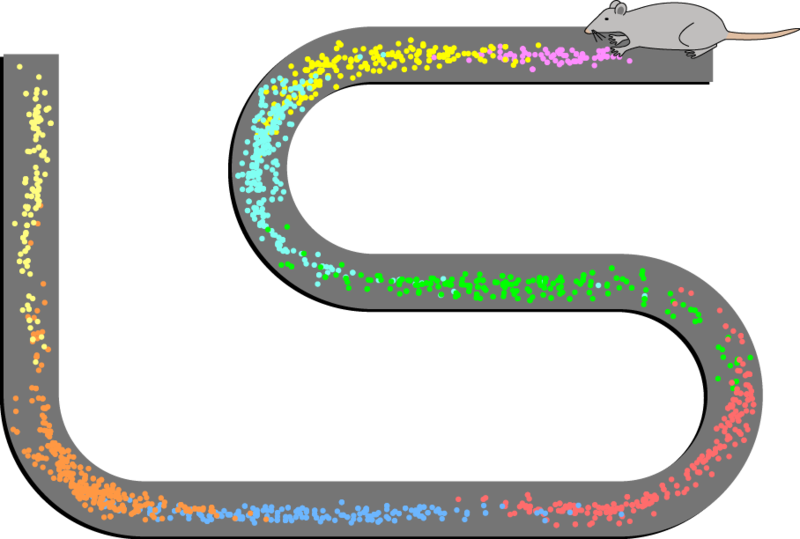
\includegraphics[width=0.9\textwidth]{Place_Cell_Spiking_Activity_Example.png}
    \end{column}
  \end{columns}	

  {\small References: \newline
  	\begin{itemize}
  	\item J. O'Keefe and J.Dostrovsky,\textit{The hippocampus as a spatial map. Preliminary evidence from unit activity in the freely-moving rat.} Brain Res. 34:171-175 (1971). 
	\item\texttt{https://commons.wikimedia.org/wiki/File:\linebreak Place\_Cell\_Spiking\_Activity\_Example.png}
	\end{itemize}}
\end{frame}
%
%
%
\begin{frame}
\frametitle{Grid cells}
\begin{columns}[T]
    \begin{column}{.5\textwidth}
			\begin{itemize}
			\item Located in  medial enthorhinal cortex (mEC). Activated at multiple spacial positions. 
			\item Firing map shows hexagonal pattern. 
			\item Mostly independent of visual stimulus
			\item Spacing, orientation, size of  patterns.
			\end{itemize}
    \end{column}
    \begin{column}{.5\textwidth}
    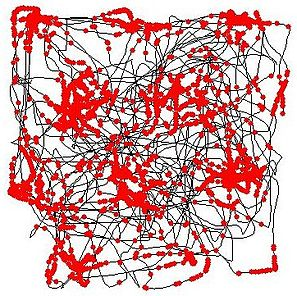
\includegraphics[width= 0.9\textwidth]{RatRunningPath.JPG}
    \end{column}
  \end{columns}
 {\small Reference: \newline
 T. Hafting, M. Fyhn, S. Molden, M.-B. Moser and E.I.Moser,\textit{Microstructure of a spatial map in the entorhinal cortex.} Nature 436: 801-806 (2005).	}
\end{frame}
%
%

%
\begin{frame}
\frametitle{Rat trajectory}
  \begin{columns}[T]
    \begin{column}{.5\textwidth}
			\begin{itemize}
		    \item Square environment of size $125 \times 125$ cm.
		    \item Speed: $v=0.4$ m/s
		    \item Every 10 ms: chose new direction from a gaussian distribution with 
		    	\begin{itemize}
		    	\item $\mu=$ previous direction
		    	\item $\sigma= 0.2$
		    	\end{itemize}
		    \end{itemize}
    \end{column}
    \begin{column}{.5\textwidth}
    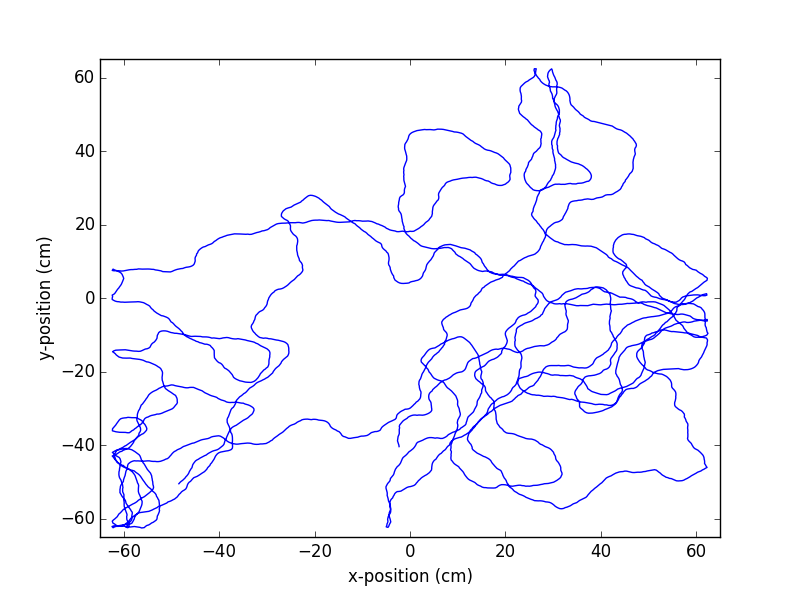
\includegraphics[width=6cm, height=6cm]{pics/running_rat.png}
    %\caption{running time: 50 seconds}
    \end{column}
  \end{columns}
\end{frame}

\begin{frame}\frametitle{Place Cells}
\begin{center}
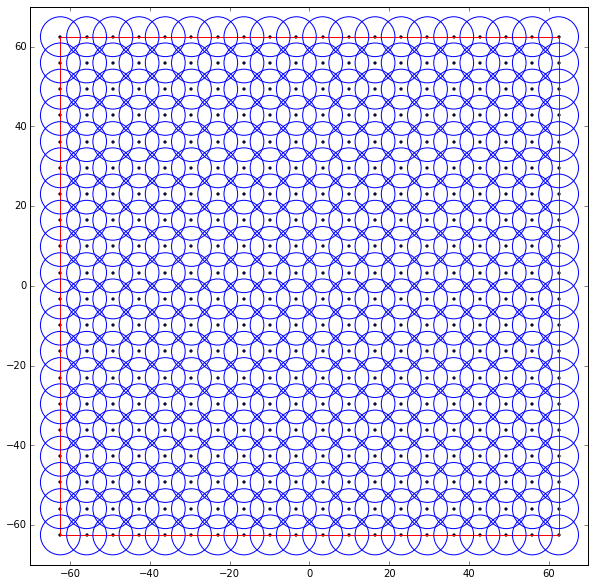
\includegraphics[scale=.3]{pics/place_cell_locations}
\end{center}
\end{frame}

\begin{frame}
\frametitle{Model: Overview}
\begin{center}
input layer output layer magic processing output
\begin{tikzpicture}[->]

	% draw input layer
	\foreach \s in {0,...,7}
	{
		\node[draw, circle] (i_\s) at (0,-\s * 0.5) {};
	}
	
	% draw output layer	
	\foreach \s in {0,...,2}
	{
		\node[draw, circle] (o_\s) at (3,-1.25 -\s * 0.5) {};
		\node[draw, circle] (m_\s) at (5,-1.25 -\s * 0.5) {};
		\path (o_\s) edge node {} (m_\s);
		\draw[->] (5.18,-1.25 -\s * 0.5) -- (6,-1.25 -\s * 0.5);
	}
	
	% draw edges
	\foreach \s in {0,...,7}
	{
			\path (i_\s) edge node {} (o_0);
	}
	\path (i_0) edge node {} (o_1);
	\path (i_0) edge node {} (o_2);

\end{tikzpicture}
\end{center}
\end{frame}

\begin{frame}
\frametitle{Model: Overview}
\begin{center}
input layer output layer magic processing output
\begin{tikzpicture}[->]

	% draw input layer
	\foreach \s in {0,...,7}
	{
		\node[draw, circle] (i_\s) at (0,-\s * 0.5) {};
	}

	\node (w) at (2, -2.7) {$w_{ij}$};	
	
	% draw output layer	
	\foreach \s in {0,...,2}
	{
		\node[draw, circle] (o_\s) at (3,-1.25 -\s * 0.5) {};
		\node[draw, circle] (m_\s) at (5,-1.25 -\s * 0.5) {};
		\path (o_\s) edge node {} (m_\s);
		\draw[->] (5.18,-1.25 -\s * 0.5) -- (6,-1.25 -\s * 0.5);
	}
	
	% draw edges
	\foreach \s in {0,...,7}
	{
			\path (i_\s) edge node {} (o_0);
	}
	\path (i_0) edge node {} (o_1);
	\path (i_0) edge node {} (o_2);

\end{tikzpicture}
\end{center}
\hskip 3cm$input_i$\hskip 2cm $output_j$\\
\hskip 3cm$i=1,...,400$\hskip 1cm $j=1,...,100$
\end{frame}
\setlength{\columnseprule}{0.4pt}

\begin{frame}
\frametitle{Model: Input Layer}
\begin{multicols}{2}
\begin{center}
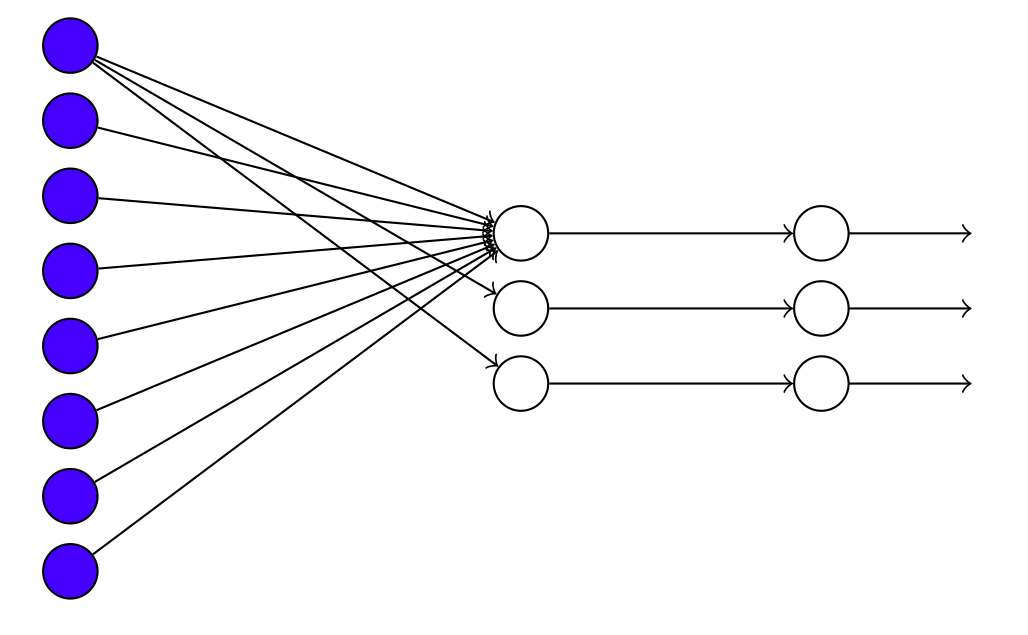
\includegraphics[scale=.1]{pics/model_input}
\vskip 2mm
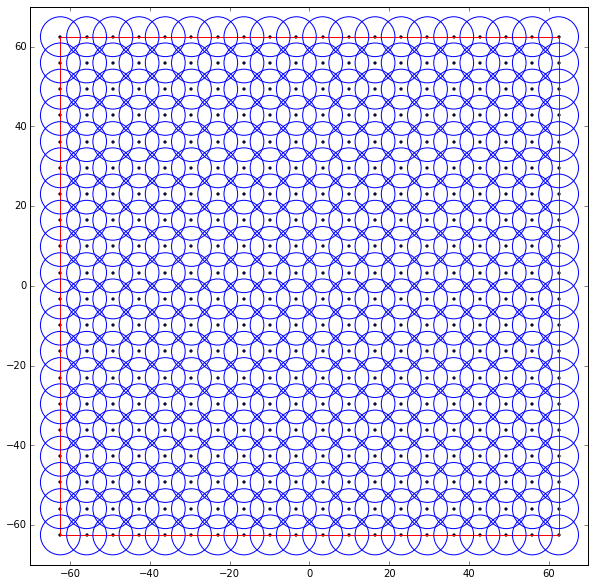
\includegraphics[scale=.15]{pics/place_cell_locations}
\end{center}
\columnbreak
\begin{center}
$input_i = \exp(-\frac{||rat - center_i||^2}{50})$
\vskip 20mm
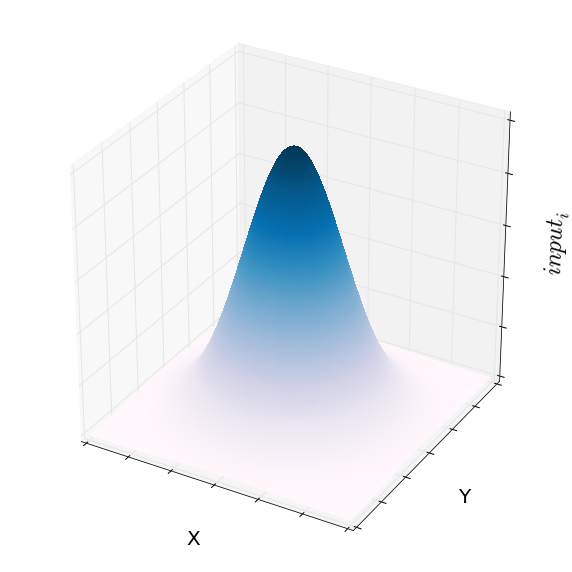
\includegraphics[scale=.3]{pics/gauss}
\end{center}
\end{multicols}
\end{frame}

\begin{frame}
\frametitle{Model: Input Layer}
\begin{multicols}{2}
\begin{center}
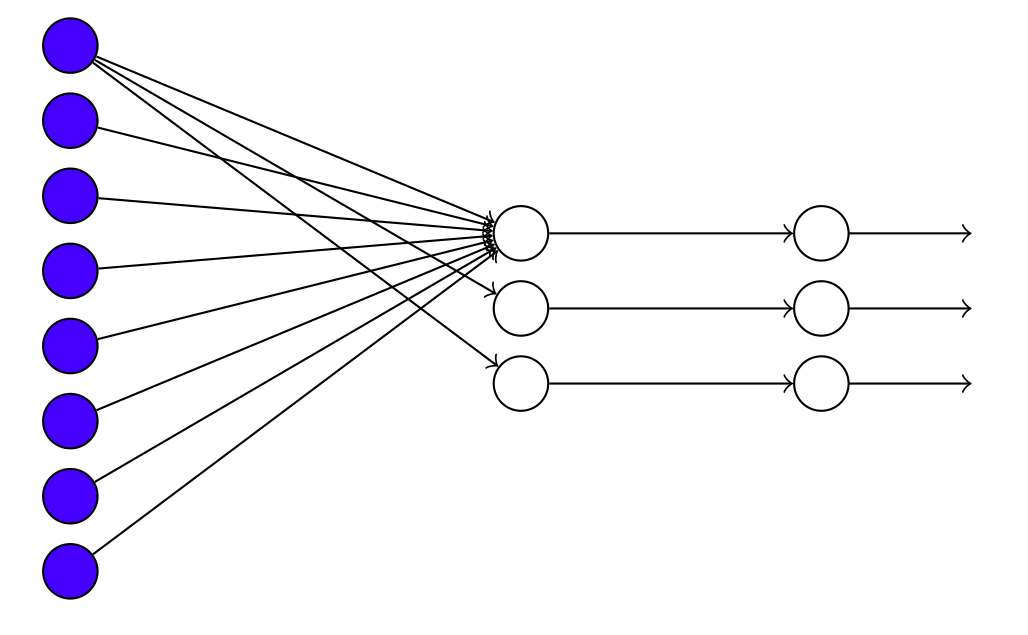
\includegraphics[scale=.1]{pics/model_input}
\vskip 2mm
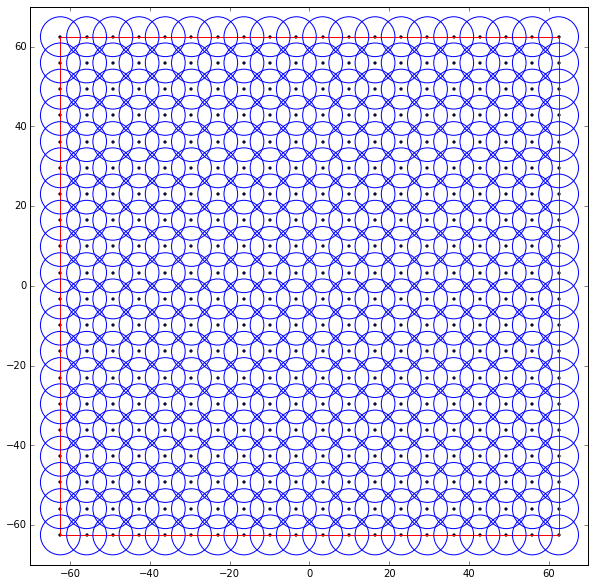
\includegraphics[scale=.15]{pics/place_cell_locations}
\end{center}
\columnbreak
\begin{center}
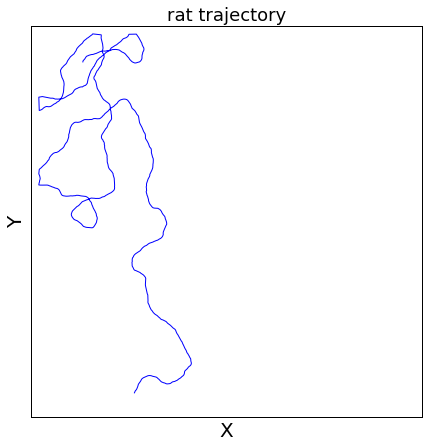
\includegraphics[scale=.3]{pics/mouse_demo}
\vskip 4mm
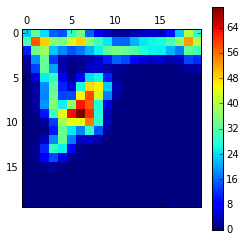
\includegraphics[scale=.4]{pics/activity_demo}
\end{center}
\end{multicols}
\end{frame}

\begin{frame}
\frametitle{Model: Output Layer}
\begin{multicols}{2}
\begin{center}
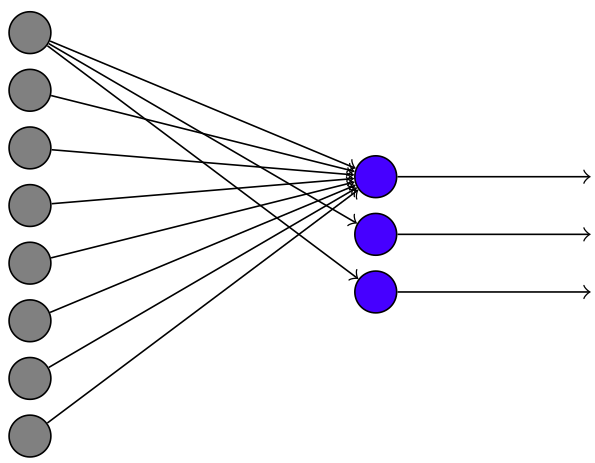
\includegraphics[scale=.1]{pics/model_output}
\end{center}
\columnbreak
\begin{center}
$h_j = \sum_i w_{ij} \cdot input_i$
\vskip 5mm
$\rightarrow$ How to determine\\ \hskip 4mm the weights $w_{ij}$?
\end{center}
\end{multicols}
\end{frame}

\begin{frame}
\frametitle{Model: Output Layer}
\begin{multicols}{2}
\begin{center}
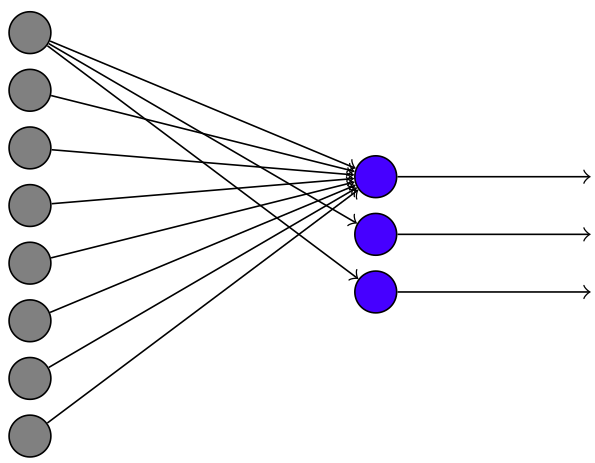
\includegraphics[scale=.1]{pics/model_output}
\end{center}
\columnbreak
\begin{center}
$h_j = \sum_i w_{ij} \cdot input_i$
\vskip 5mm
$\rightarrow$ How to determine\\ \hskip 4mm the weights $w_{ij}$?\\
$\rightarrow$ Hebbian learning dynamics\\
\end{center}
\end{multicols}
\end{frame}

\begin{frame}
\frametitle{Model: Output Layer}
\begin{multicols}{2}
\begin{center}
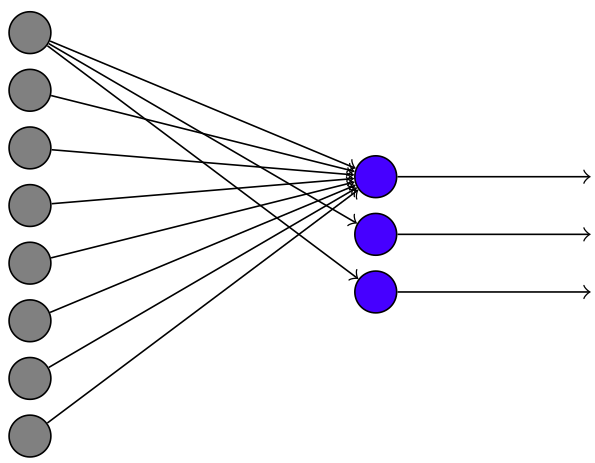
\includegraphics[scale=.1]{pics/model_output}
\end{center}
\columnbreak
\begin{center}
$h_j = \sum_i w_{ij} \cdot input_i$
\vskip 5mm
$\rightarrow$ How to determine\\ \hskip 4mm the weights $w_{ij}$?\\
$\rightarrow$ Hebbian learning dynamics\\
\hskip 7mm 'Fire together, wire together'\\
$\rightarrow$ Details on that in 2 slides
\end{center}
\end{multicols}
\end{frame}

\begin{frame}
\frametitle{Model: Processing}
\begin{multicols}{2}
\begin{center}
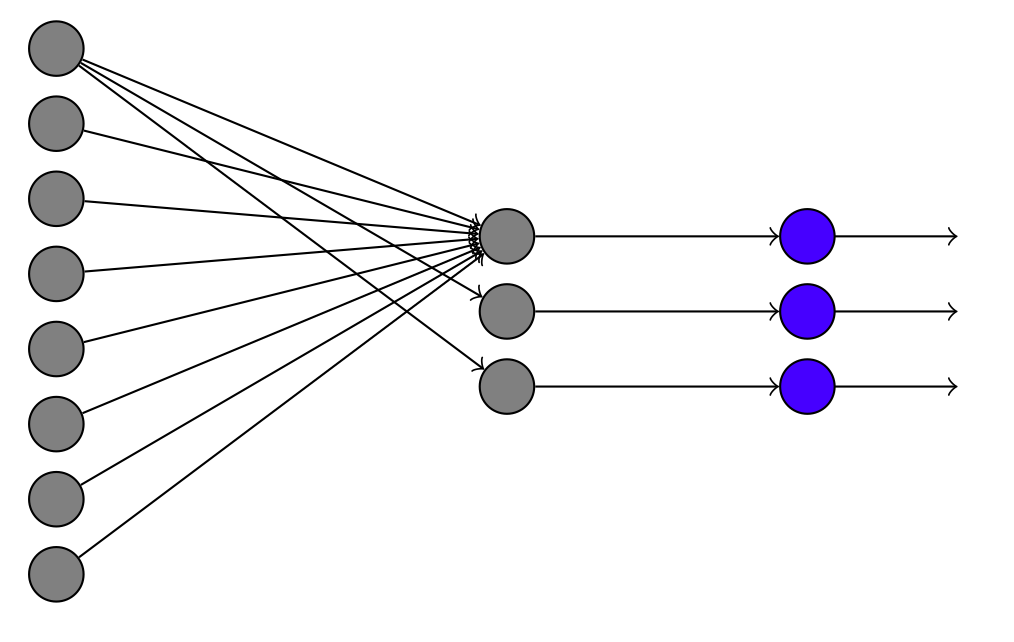
\includegraphics[scale=.1]{pics/model_processing}
\end{center}
\columnbreak
\begin{center}
$h_j(t) = \sum_i w_{ij} \cdot input_i(t)$\\
\vskip 6mm
$\rightarrow$ adaptation dynamics:\\
\vskip 3mm
$\tau^+\frac{d}{dt}r^+_j=h_j(t)-r^+_j(t)-r^-_j(t)$\\
\vskip 3mm
$\tau^-\frac{d}{dt}r^-_j(t)=r^-_j(t)$
\vskip 5mm
\end{center}
\end{multicols}
\end{frame}

\begin{frame}
\frametitle{Model: Processing}
\begin{multicols}{2}
\begin{center}
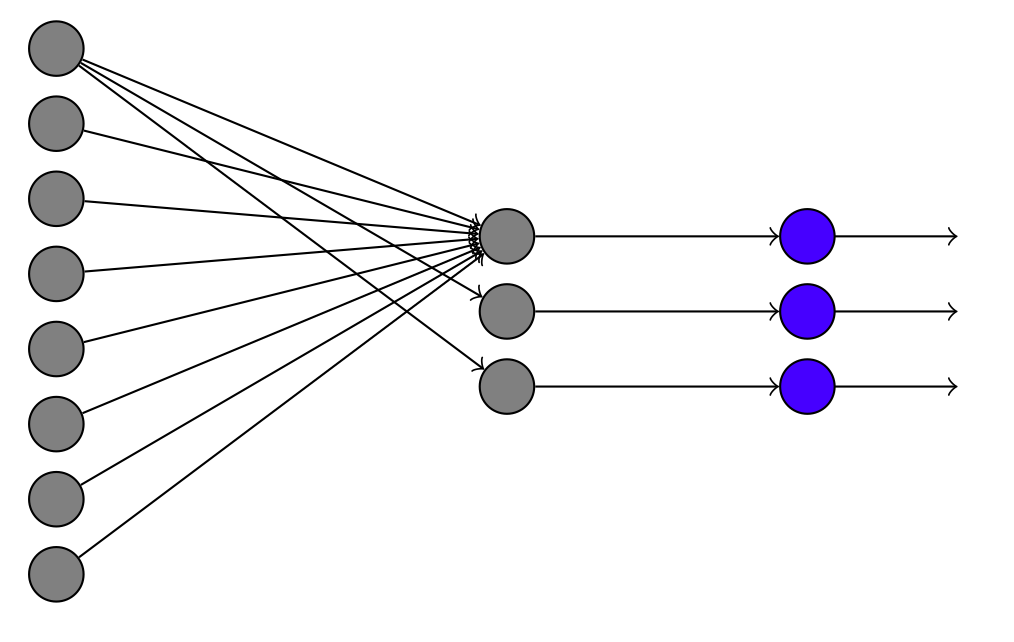
\includegraphics[scale=.1]{pics/model_processing}
\vskip 3mm
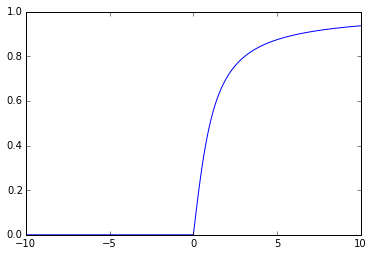
\includegraphics[scale=.3]{pics/output_function}
\end{center}
\columnbreak
\begin{center}
$h_j(t) = \sum_i w_{ij} \cdot input_i(t)$\\
\vskip 6mm
$\rightarrow$ adaptation dynamics:\\
\vskip 3mm
$\tau^+\frac{d}{dt}r^+_j=h_j(t)-r^+_j(t)-r^-_j(t)$\\
\vskip 3mm
$\tau^-\frac{d}{dt}r^-_j(t)=r^-_j(t)$\\
\vskip 3mm
$\rightarrow$ output:\\
\vskip 3mm
$output_j(t)=\frac{2}{\pi} \arctan (g \cdot (r^+_j(t)-\mu)) \cdot \theta(r_j^+(t)-\mu)$\\
\vskip 3mm
$g$ - gain, $\mu$ - threshold
\end{center}
\end{multicols}
\end{frame}

\begin{frame}
\frametitle{Model: Weight Updates}
\begin{multicols}{2}
\begin{center}
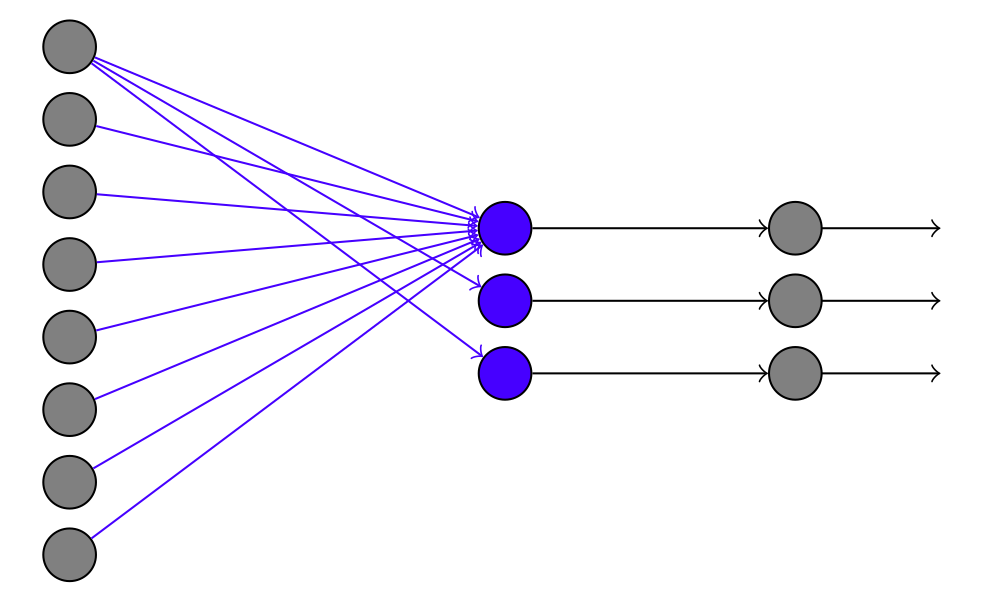
\includegraphics[scale=.1]{pics/model_output_2}
\end{center}
\columnbreak
\begin{center}
$h_j = \sum_i w_{ij} \cdot input_i$
\vskip 5mm
$\rightarrow$ How to determine\\ \hskip 4mm the weights $w_{ij}$?\\
$\rightarrow$ Hebbian learning dynamics\\
\vskip 4mm
$w_{ij}(t+\Delta)=w_{ij}(t)+$\\
$ \epsilon (input_i(t)\cdot output_j - \sum_s input_i (s) \cdot \sum_s output_j(s))$
\end{center}
\end{multicols}
\end{frame}

\begin{frame}
\frametitle{Cherrypicked final weights}
\begin{columns}[t]
\column{.5\textwidth}
\centering
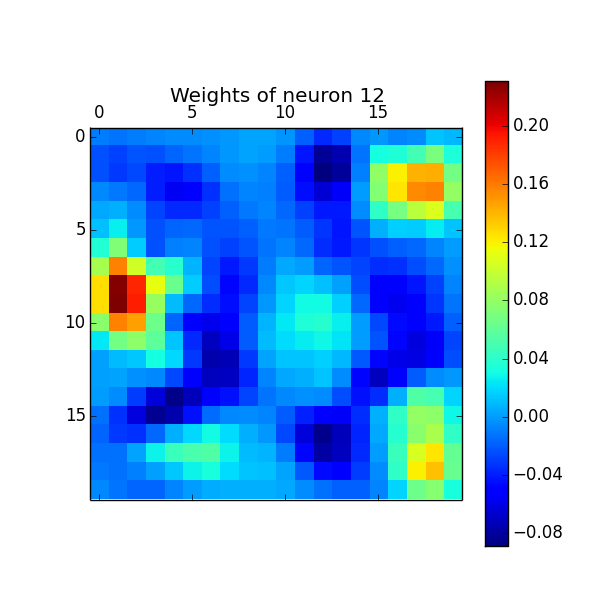
\includegraphics[width=4cm,height=4cm]{neurons/neuron_w_12.png}\\
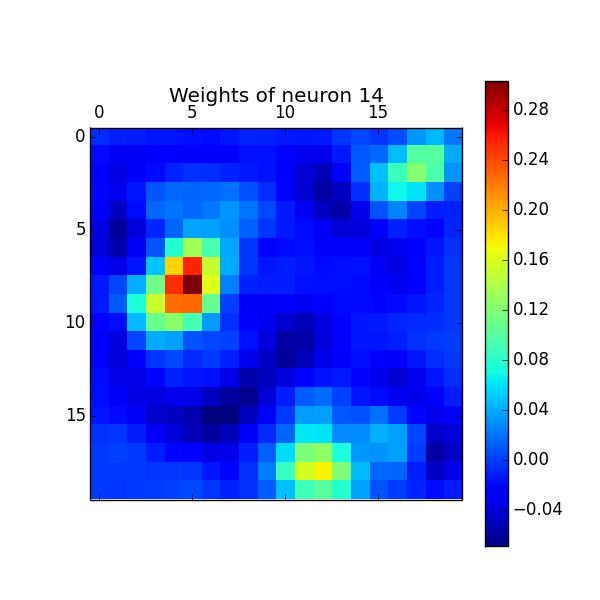
\includegraphics[width=4cm,height=4cm]{neurons/neuron_w_14.png}
\column{.5\textwidth}
\centering
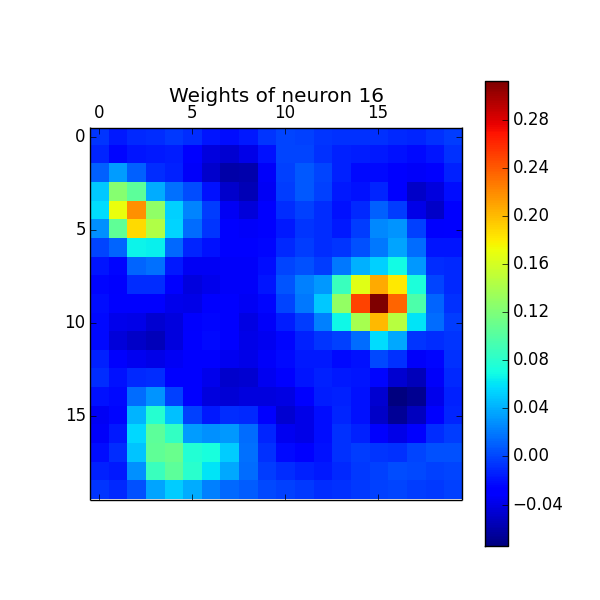
\includegraphics[width=4cm,height=4cm]{neurons/neuron_w_16.png}\\
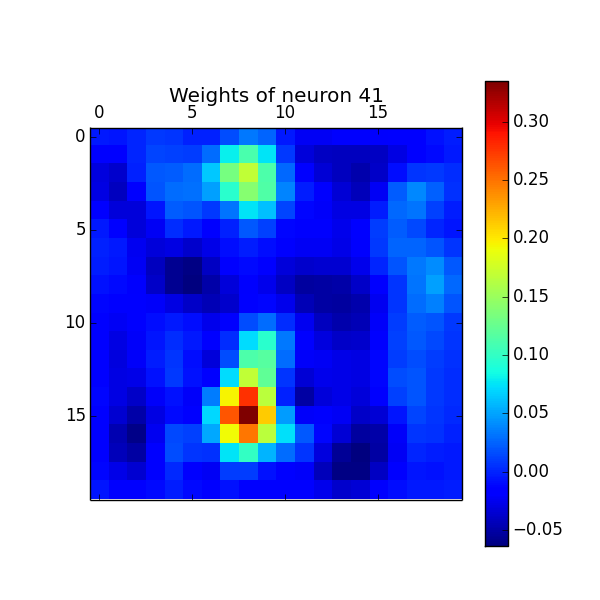
\includegraphics[width=4cm,height=4cm]{neurons/neuron_w_41.png}
\end{columns}
\end{frame}

\begin{frame}
\frametitle{Cherrypicked final autocorrelations}
\begin{columns}[t]
\column{.5\textwidth}
\centering
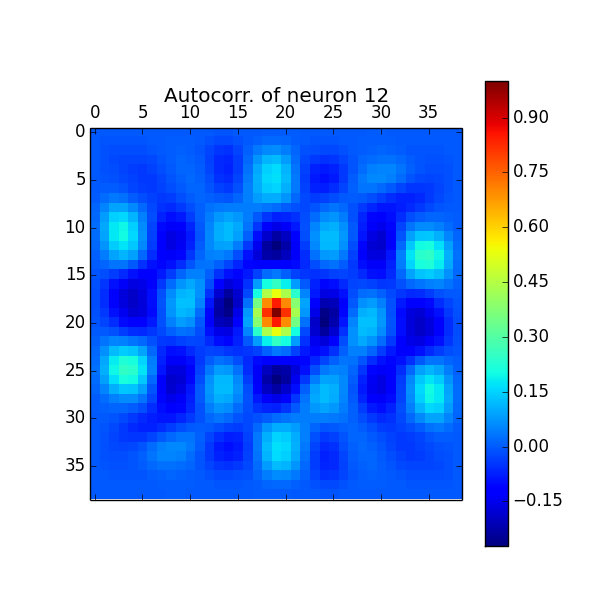
\includegraphics[width=4cm,height=4cm]{neurons/neuron_a_12.png}\\
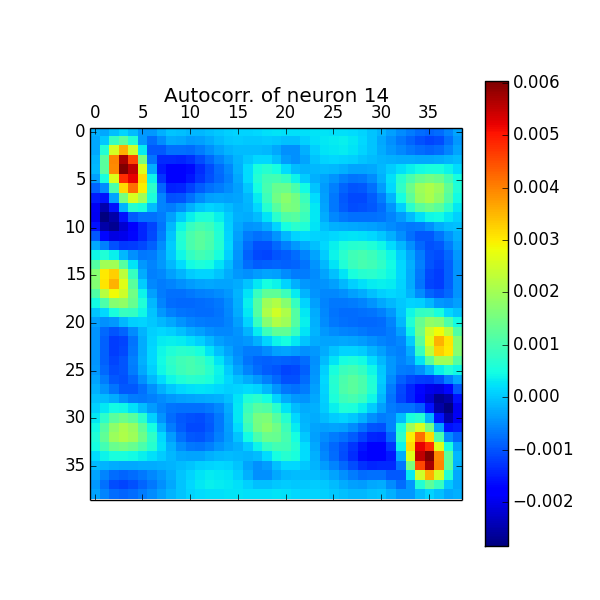
\includegraphics[width=4cm,height=4cm]{neurons/neuron_a_14.png}
\column{.5\textwidth}
\centering
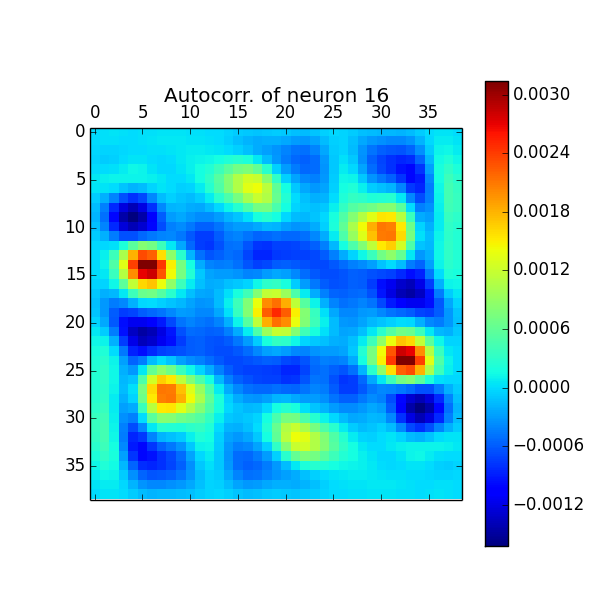
\includegraphics[width=4cm,height=4cm]{neurons/neuron_a_16.png}\\
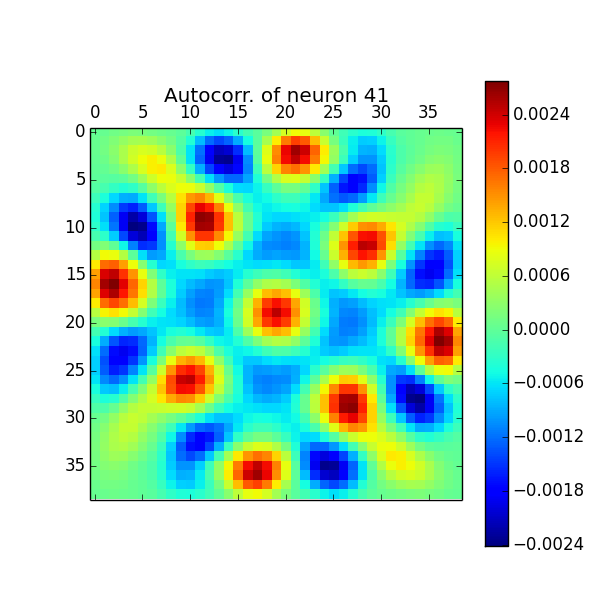
\includegraphics[width=4cm,height=4cm]{neurons/neuron_a_41.png}
\end{columns}
\end{frame}

\begin{frame}
\frametitle{Time evolution of weights for a neuron}
\begin{columns}[t]
\column{.5\textwidth}
\centering
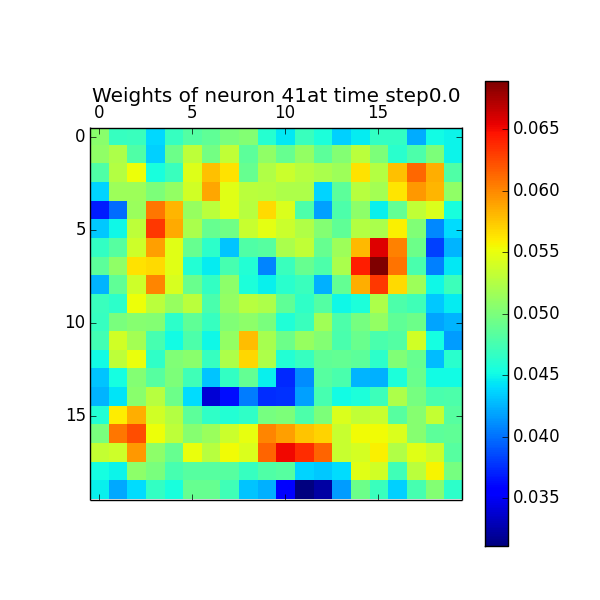
\includegraphics[width=6cm,height=6cm]{neurons/neuron_w_41_t_0.png}\\
\column{.5\textwidth}
\centering
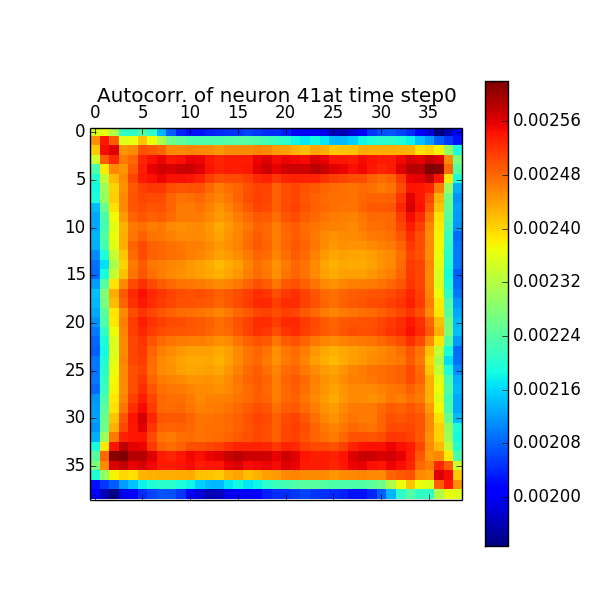
\includegraphics[width=6cm,height=6cm]{neurons/neuron_a_41_t_0.png}\\
\end{columns}
\end{frame}

\begin{frame}
\frametitle{Time evolution of weights for a neuron}
\begin{columns}[t]
\column{.5\textwidth}
\centering
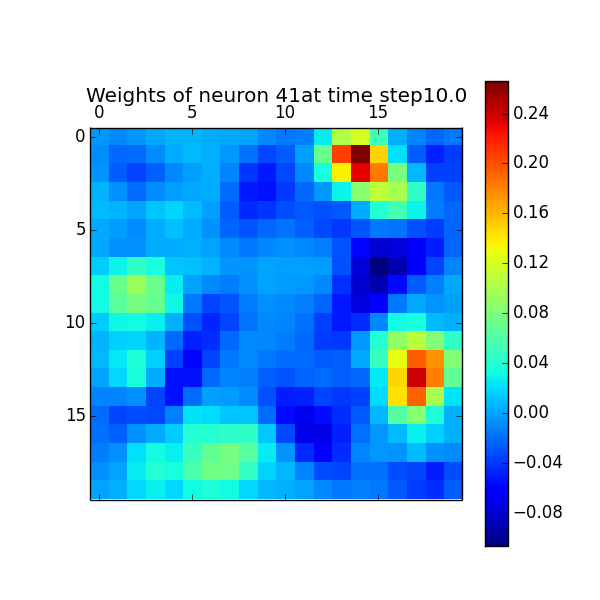
\includegraphics[width=6cm,height=6cm]{neurons/neuron_w_41_t_10.png}\\
\column{.5\textwidth}
\centering
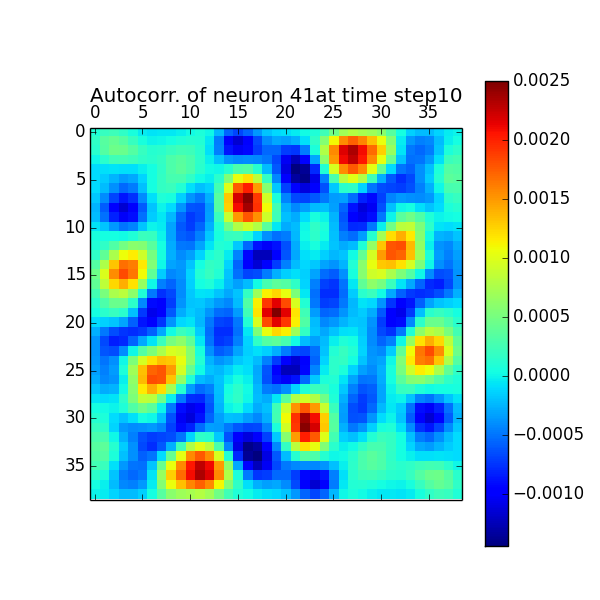
\includegraphics[width=6cm,height=6cm]{neurons/neuron_a_41_t_10.png}\\
\end{columns}
\end{frame}

\begin{frame}
\frametitle{Time evolution of weights for a neuron}
\begin{columns}[t]
\column{.5\textwidth}
\centering
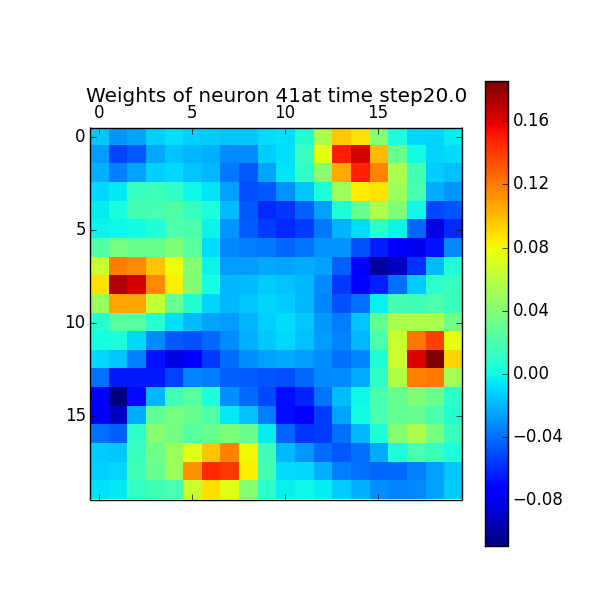
\includegraphics[width=6cm,height=6cm]{neurons/neuron_w_41_t_20.png}\\
\column{.5\textwidth}
\centering
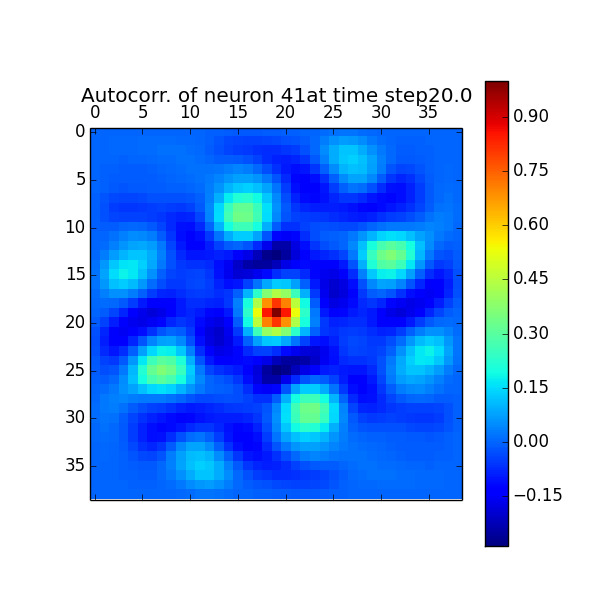
\includegraphics[width=6cm,height=6cm]{neurons/neuron_a_41_t_20.png}\\
\end{columns}
\end{frame}


\begin{frame}
\frametitle{Time evolution of weights for a neuron}
\begin{columns}[t]
\column{.5\textwidth}
\centering
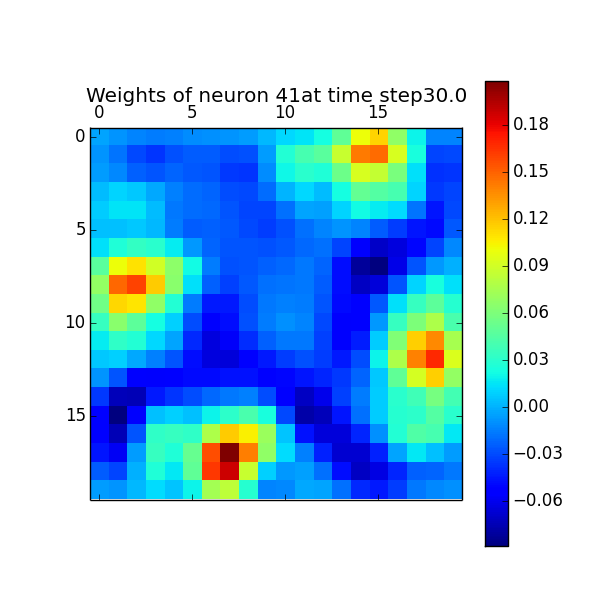
\includegraphics[width=6cm,height=6cm]{neurons/neuron_w_41_t_30.png}\\
\column{.5\textwidth}
\centering
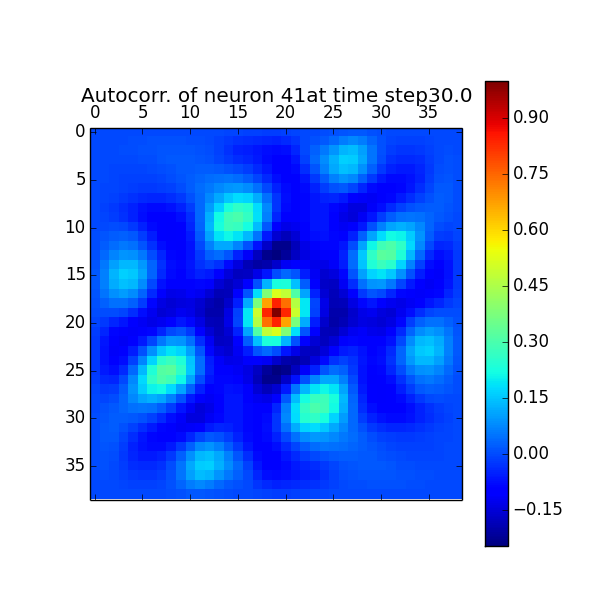
\includegraphics[width=6cm,height=6cm]{neurons/neuron_a_41_t_30.png}\\
\end{columns}
\end{frame}

\begin{frame}
\frametitle{Time evolution of weights for a neuron}
\begin{columns}[t]
\column{.5\textwidth}
\centering
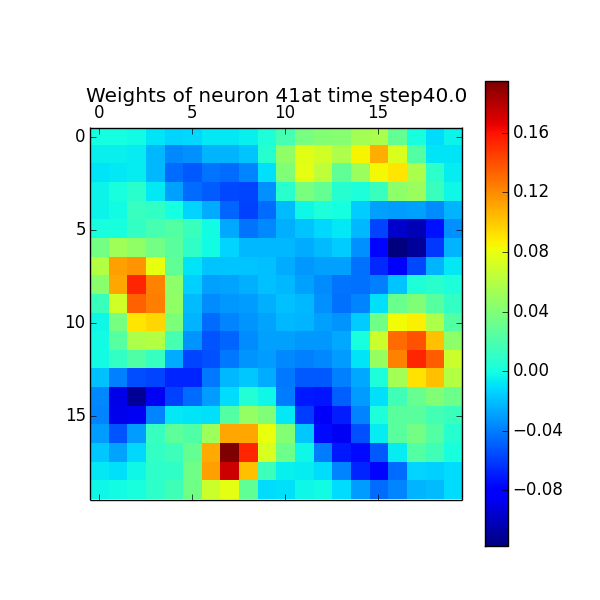
\includegraphics[width=6cm,height=6cm]{neurons/neuron_w_41_t_40.png}\\
\column{.5\textwidth}
\centering
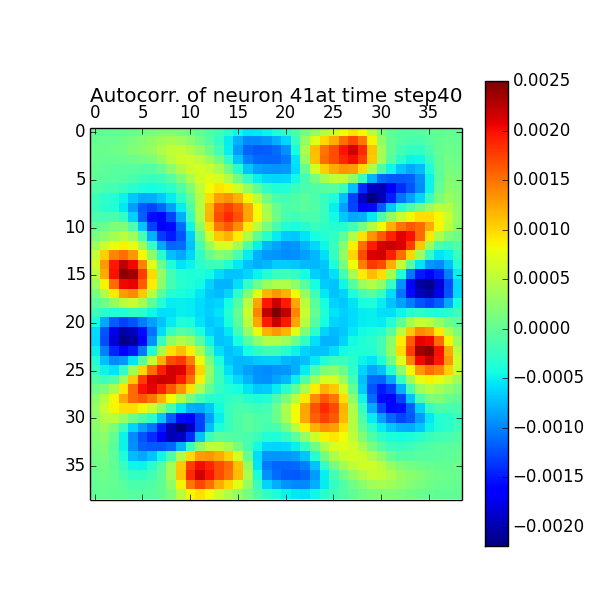
\includegraphics[width=6cm,height=6cm]{neurons/neuron_a_41_t_40.png}\\
\end{columns}
\end{frame}

\begin{frame}
\frametitle{Time evolution of weights for a neuron}
\begin{columns}[t]
\column{.5\textwidth}
\centering
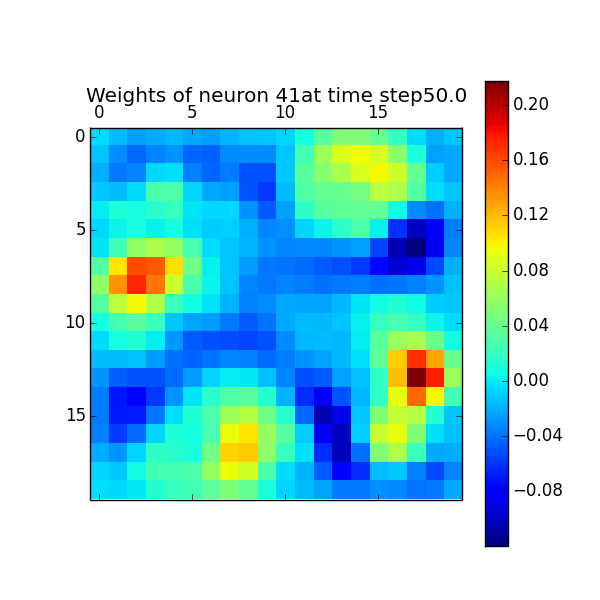
\includegraphics[width=6cm,height=6cm]{neurons/neuron_w_41_t_50.png}\\
\column{.5\textwidth}
\centering
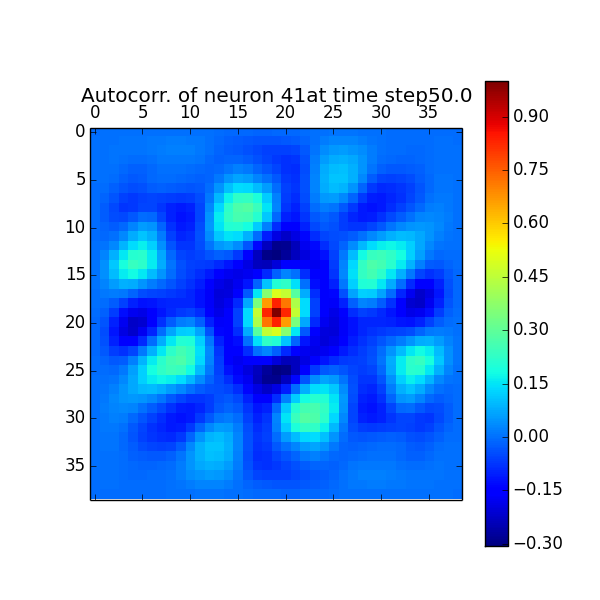
\includegraphics[width=6cm,height=6cm]{neurons/neuron_a_41_t_50.png}\\
\end{columns}
\end{frame}

\begin{frame}
\frametitle{Time evolution of weights for a neuron}
\begin{columns}[t]
\column{.5\textwidth}
\centering
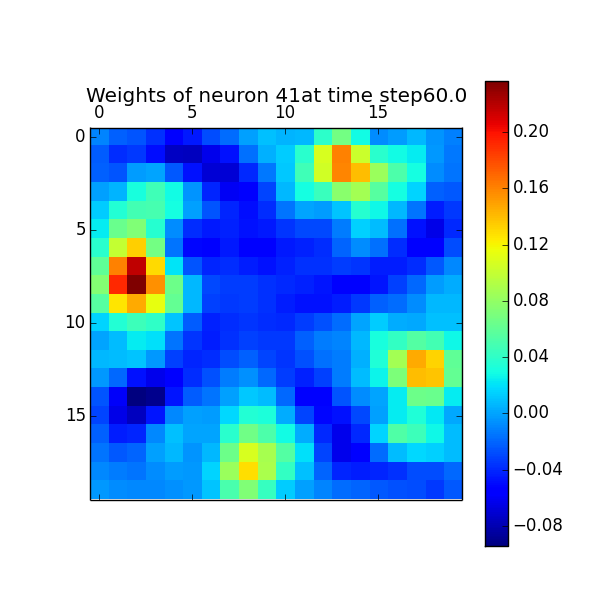
\includegraphics[width=6cm,height=6cm]{neurons/neuron_w_41_t_60.png}\\
\column{.5\textwidth}
\centering
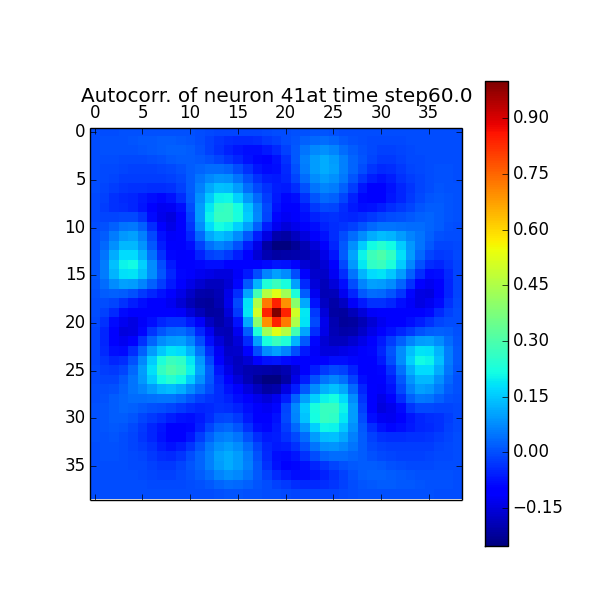
\includegraphics[width=6cm,height=6cm]{neurons/neuron_a_41_t_60.png}\\
\end{columns}
\end{frame}

\begin{frame}
\frametitle{Time evolution of weights for a neuron}
\begin{columns}[t]
\column{.5\textwidth}
\centering
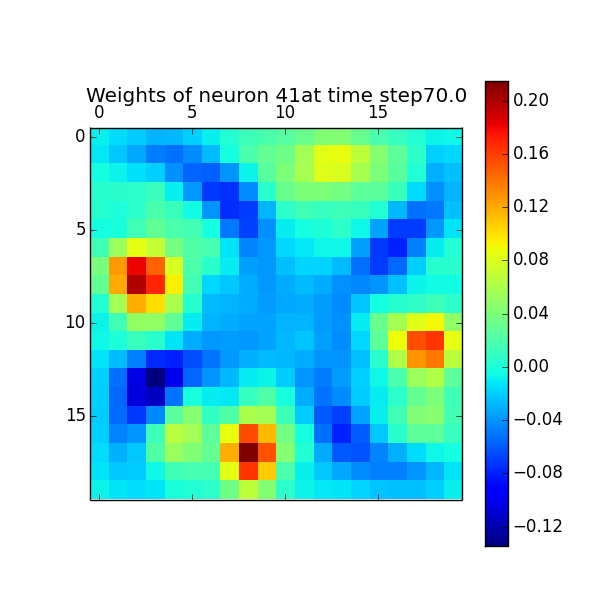
\includegraphics[width=6cm,height=6cm]{neurons/neuron_w_41_t_70.png}\\
\column{.5\textwidth}
\centering
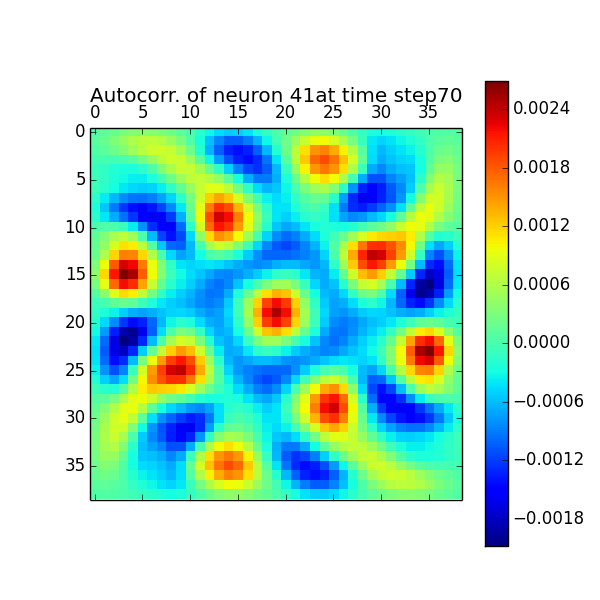
\includegraphics[width=6cm,height=6cm]{neurons/neuron_a_41_t_70.png}\\
\end{columns}
\end{frame}

\begin{frame}
\frametitle{Time evolution of weights for a neuron}
\begin{columns}[t]
\column{.5\textwidth}
\centering
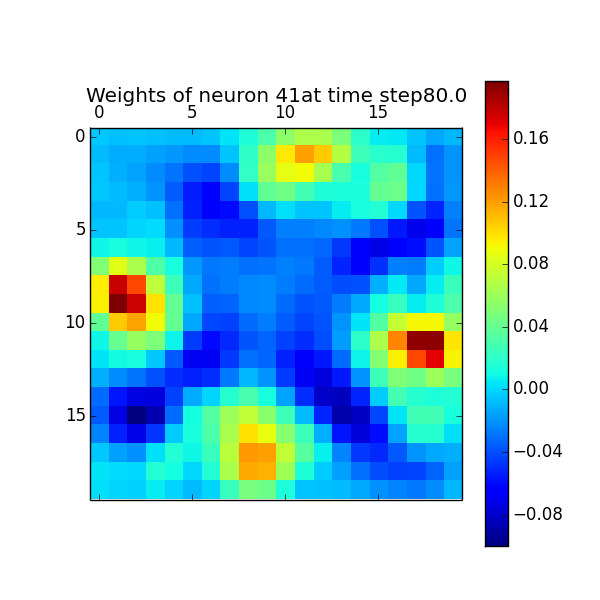
\includegraphics[width=6cm,height=6cm]{neurons/neuron_w_41_t_80.png}\\
\column{.5\textwidth}
\centering
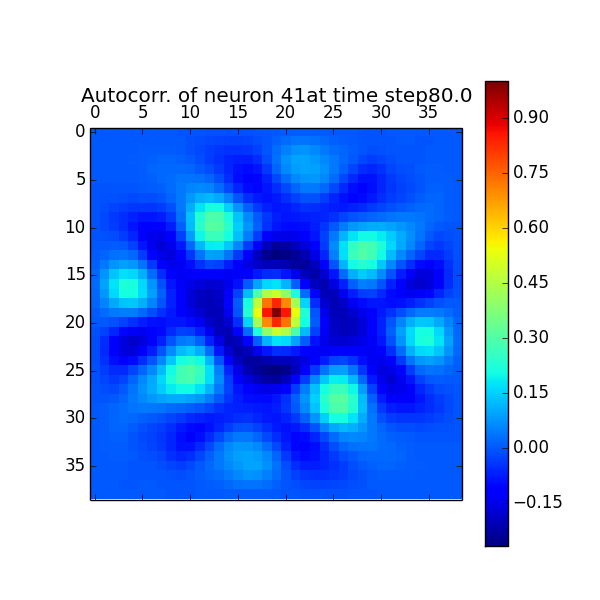
\includegraphics[width=6cm,height=6cm]{neurons/neuron_a_41_t_80.png}\\
\end{columns}
\end{frame}

\begin{frame}
\frametitle{Time evolution of weights for a neuron}
\begin{columns}[t]
\column{.5\textwidth}
\centering
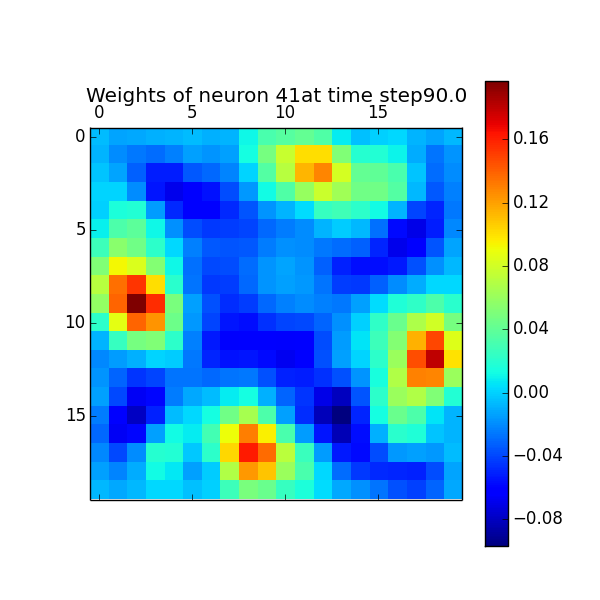
\includegraphics[width=6cm,height=6cm]{neurons/neuron_w_41_t_90.png}\\
\column{.5\textwidth}
\centering
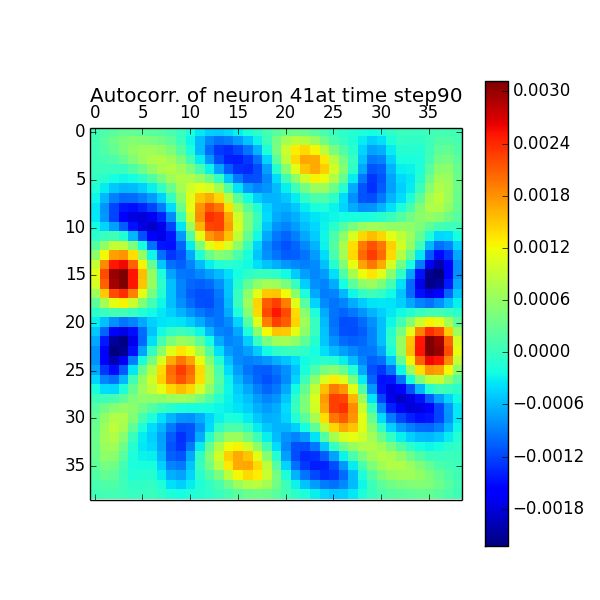
\includegraphics[width=6cm,height=6cm]{neurons/neuron_a_41_t_90.png}\\
\end{columns}
\end{frame}

\begin{frame}
\frametitle{Time evolution of weights for a neuron}
\begin{columns}[t]
\column{.5\textwidth}
\centering
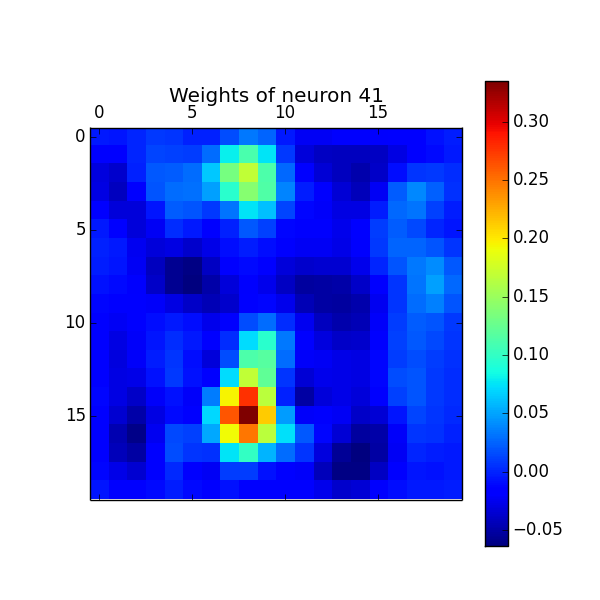
\includegraphics[width=6cm,height=6cm]{neurons/neuron_w_41.png}\\
\column{.5\textwidth}
\centering
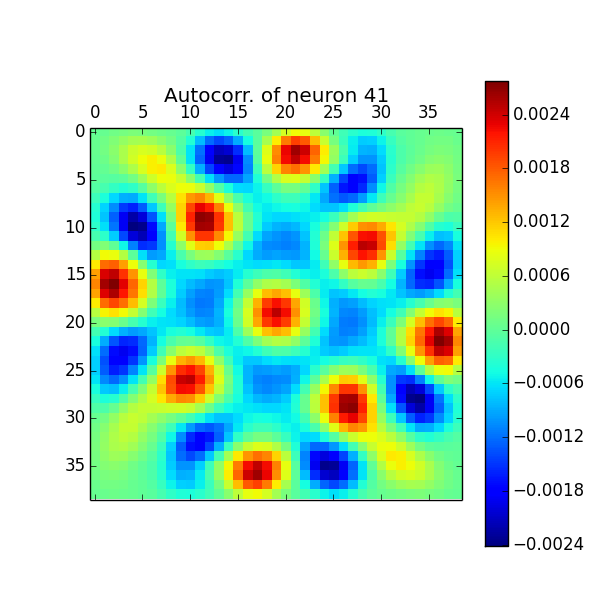
\includegraphics[width=6cm,height=6cm]{neurons/neuron_a_41.png}\\
\end{columns}
\end{frame}



\end{document}
%